\section{Background}
\label{sec:background}
Node.js is a JavaScript run-time environment that executes code outside of a browser. Node.js is built on Google's V8 JavaScript engine where the V8 is written in C++ and used to compile JavaScript code directly to native machine code before executing it. 
The technology also allows the user to create Web servers and networking tools using JavaScript and a collection of 'modules' that are used to handle various core functionality. 
\cite{wiki:nodejs}.

\subsection{Package Manager: Node Package Module}
As mentioned, Node.js allows the user to use a collection of modules for different tasks. They are installed from Node Package Module which is one of the most powerful tools of Node.js. The modules are installed from the command "npm install modulename" and the modules are downloaded to folder "{node\_modules}". Node Package Module started as a way to download dependencies, but has quickly become an important tool for working with JavaScript. The idea of npm modules is to have a set of reusable components that is available through an easy installation via an online repository that can be found at the npm website. \cite{npm:webpage}
\\\\
Every Node.js project comes with an package.json file. This file is the core of the Node.js ecosystem and describes what modules are required for a project. It manages modules of a project and also scripts for generating builds and running tests \cite{npmjs:modules}. 
The package.json file has some important properties that must be initialized before one can start on the project such as name, version, scripts and dependencies. 
\begin{figure}[h!]
  \centering
  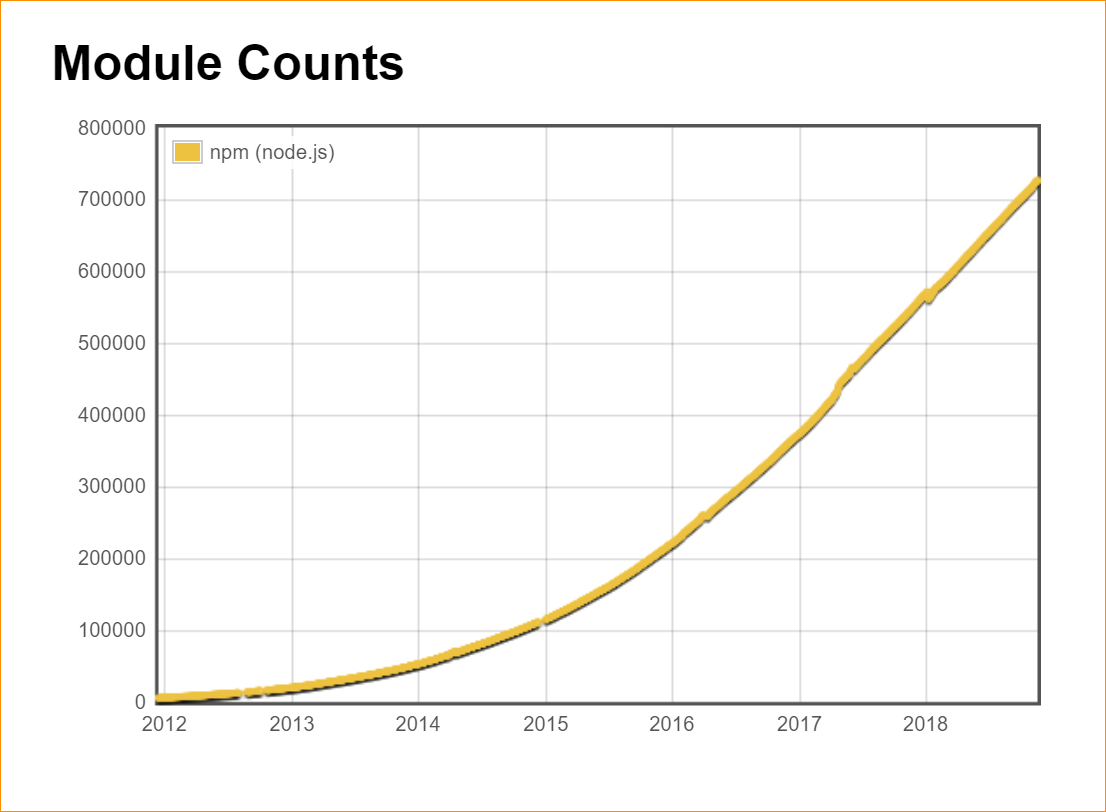
\includegraphics[scale=0.5]{figs/npmmodulescounts.png}
  \caption{How the number of modules have grown over the years \cite{image:modulecount}}
\end{figure}\\
One of the reasons why npm and Node.js became popular is because of how simple it is for developers to create new packages and how easy it is for others to use them. From figure 1 we can see that number of modules in npm has grown almost polynomial since its start. 
\\\\
Some of the most useful modules that we use in our prototype: 
\begin{itemize}
    \item Express: Web development framework (server) for Node.js and a standard for most Node.js applications.
    \item body-parser: A module that goes in hand with Express. Extracts the entire body of an incoming request stream from Express. Makes it easy to use JSON.
    \item Mongo/Mongoose: Wrappers to interact with MongoDB database in Node.js
    \item Socket.io: Real-time bidirectional event-based communication.  
\end{itemize}

\subsection{Single Thread and Event Loop}
Node.js uses 'Single Threaded Event Loop Model' architecture to handle multiple concurrent tasks versus other web application technologies like JSP, SPRING, HTML, etc., that follow 'Multi-Threaded Request-Response' architecture to handle multiple concurrent clients. 
\\\\
To compare, an example of a more traditional solution is a PHP application on an Apache server. Both Node.js and PHP can be used to to build network programs such as Web servers. The main difference between these technologies is that most functions in PHP block until termination, while functions in Node.js are non-blocking. This means that commands execute concurrently or even in parallel and use callbacks to signal completion (or failure). 
\\\\
Node.js works on a single thread because it uses non-block I/O calls. It allows the server to support multiple concurrent connections and the connections are held in an event loop, hence event-driven system.
It also optimizes throughout and scalability in web applications with many I/O operations, making Node.js applications extremely fast and efficient. \cite{docs:eventloop}

\begin{figure}[h!]
  \centering
  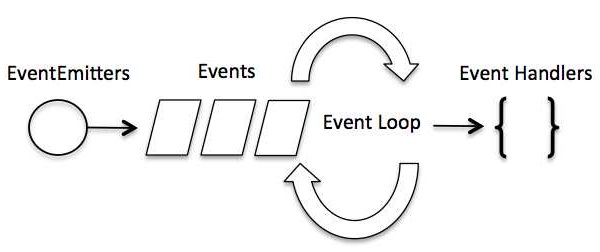
\includegraphics[scale=0.5]{figs/event_loop.jpg}
  \caption{Event Loop with an Event Emitter which listen to incoming events \cite{eventloop:image}}
\end{figure}

The design of using single thread event loop and sharing this thread among all the client is intended for building highly concurrent applications, where any function performing I/O must use a callback. A callback is a function that is to be executed after another function has finished executing \cite{codeburst:callback}. 
\\\\
Despite JavaScript being single-threaded, Node.js uses event loop to handle scalability instead of threads. With the event loop it is easier to handle multiple clients because there is no need to create more threads, and since Node.js uses less threads, it can utilize on less resources or memory. 
\\\\
When the Node.js server starts, the event loop get initialized and simply waits for events to occur. The event loop has an EventEmitter class that listens for events and triggers a callback function when an event is detected. 

\subsection{V8}
V8 engine is a open source JavaScript engine provided by Google. It is a engine that converts JavaScript code into lower level that microprocessors can understand. The V8 can run JavaScript standalone, but at we can also add our own function implementation to the engine.

\begin{figure}[h!]
  \centering
  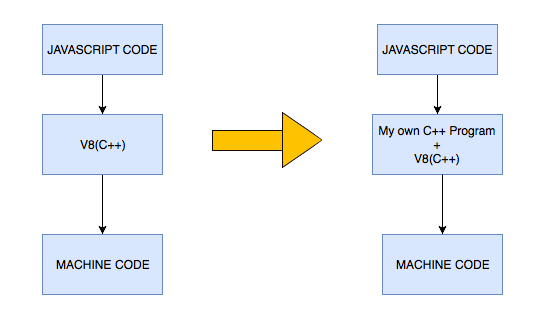
\includegraphics[scale=0.5]{figs/v8engine.png}
  \caption{Traditional Thread Solution vs. Node.js' Single Thread
  \cite{article:v8engine}}
\end{figure}

The V8 engine is written in C++ and Node.js in itself is a C++ implementation of the engine allowing server side programming and networking applications, and what Ryan Dahl did to achieve Node.js was that he added event I/O architecture, network- and HTTP-I/O libraries to the V8 engine. \cite{article:v8engine}

\subsection{Technology comparison to Java EE}
As we can see, Node.js is a well built technology, but how does it compare to the technology used in our previous project, Java EE? 
\\\\
Java EE uses standard Java as a language, which has a solid foundation and strong typing. Java EE applications often end up being very robust and resilient, much more so than an application created in JavaScript. But there are several reasons that JavaScript is one of the most popular languages in the world right now, one of the biggest reasons being it's simplicity compared to Java. Node.js utilizes this already simple language on both frontend and backend, resulting in a very simple development experience. 
\\\\
There is a lot of libraries and official documentation for Java EE, e.g., Oracle for documentation and Maven repository for libraries. The same goes for Node.js, which has the worlds biggest software registry at it's fingertips thanks to npm. Npm has become a very powerful tool for any JavaScript developer, even without Node.js. There is also a lot of official documentation for Node.js just like Java EE (though the Java EE documentation is much more mundane), but there is more relevant help to find online for Node.js (tutorials, forums, videos etc.), due to it's popularity.
\\\\
As mentioned earlier, Node.js creates a new single thread for handling concurrent function calls, whereas Java EE uses multithreading. Creating multiple threads may use extra time and memory, but it prevents complete blocking if a deadlock appears and it doesn't starve other threads if one is running slowly. It is worth noting that deadlocks are highly unlikely in Node.js because of non I/O blocking, which makes the technology more scalable, just like Java EE. \cite{compare:javanode} 
\\\\
As we have illustrated these two technologies have both similarities and differences. Both technologies are supposedly simple, powerful and versatile, but Java EE is also more robust. One is not necessarily better than the other and different applications have different needs, so the developer has to decide which language to use. Luckily we have been working with both technologies, and can hopefully give a good "in practice" comparison between the two when we examine our prototype. 